\begin{figure}
    \centering
    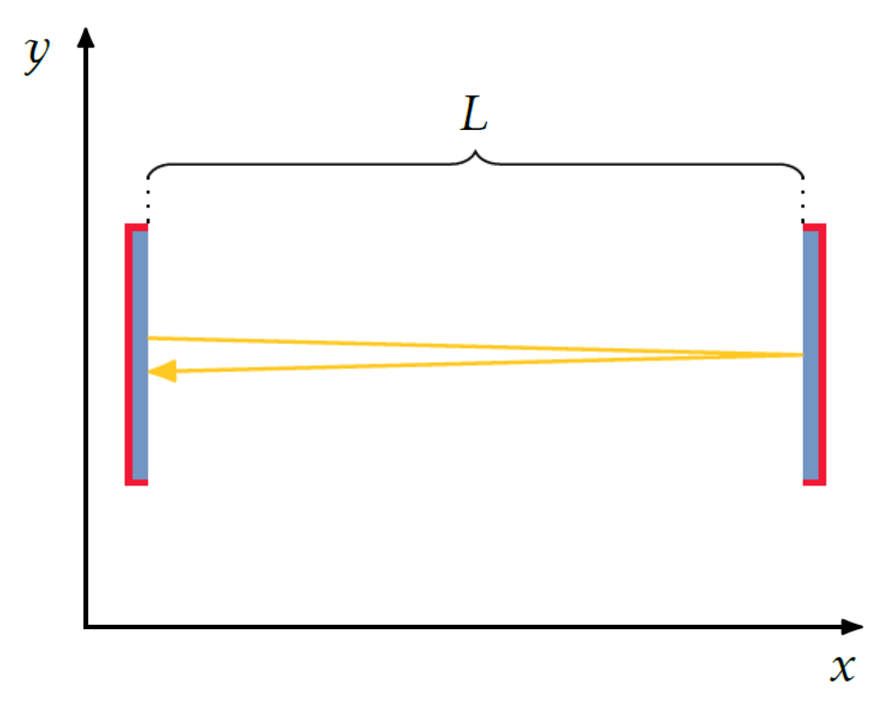
\includegraphics[width = .6\columnwidth]{SR/billeder/lysur.eps}
    \caption{Det roterede lysur i sit hvilesystem. For observatører bevæger uret sig i $x$-retningen. Kilde: figur 2.1 \cite{uggerhojSpecielRelativitetsteori2016}.}
    \label{fig:roteret_lysur}
\end{figure}
%
\section{Længdeforkortelse} \label{sec:Laengdeforkortelse}
Ligesom tiden forløber forskelligt for forskellige observatører, vil afstande også observeres forskelligt.
Lad os vende tilbage til lysuret, med den detalje at vi nu drejer uret \SI{90}{\degree}, således at lyset bevæger sig parallelt med urets bevægelsesretning, se figur \ref{fig:roteret_lysur}. I hvile er perioden for lysuret
\begin{equation}
    T_0=\frac{2L_0}{c} \: .
\end{equation}
Urets periode, set fra observatøren, skal deles op i to dele, den ene, hvor lyset rejser i samme retning som lysuret, og en anden hvor de rejser i hver sin retning\footnote{Retningen af uret afhænger af observatøren.}.
Perioden er så
\begin{equation}
    T=\frac{L}{c+v}+\frac{L}{c-v}=\frac{L(c-v+c+v)}{c^2-v^2}=\frac{2cL}{c^2-v^2}=\frac{2L}{c(1-v^2/c^2)}=\frac{2\gamma^2 L}{c} \: .
\end{equation}
Sammenhængen imellem et lysur i hvile og et i bevægelse er $T=\gamma T_0$ så sætter vi de perioder vi lige har fundet ind, og isolerer længderne får vi
\begin{align}
T&=\gamma T_0\\
\Rightarrow \frac{2L\gamma^2}{c}&=\gamma\frac{2L_0}{c}\\
\Rightarrow L&=\frac{L_0}{\gamma}=\sqrt{1-\frac{v^2}{c^2}}L_0 \: . \label{rel:Laengdeforkortelse}
\end{align}
Ligesom tiden går langsommere for et objekt i bevægelse, så vil objektet også virke sammentrukket langs bevægelsesretningen set fra en observatør i hvile. Set fra objektet i bevægelse vil verden omkring det være sammentrykket i bevægelsesretningen.

Vender vi tilbage til myonerne, vil afstanden de skal tilbagelægge for at nå Jordens overflade være langt mindre, idet verden trækkes sammen i bevægelsesretningen for et objekt i bevægelse.
Man kan også observere længdeforkortning andre steder. Et eksempel er indenfor elektronkrystallografi. Her sender man elektroner ind imod en krystal. Jo højere hastighed man sender elektronerne ind med, desto mere komprimeret virker krystallen.